\chapter{Судалгаа}

Машин сургалт тэр дундаа гар бичмэл танилттай холбоотой машин сургалтын өгөгдлийг хэрхэн бэлтгэх, зохион байгуулах тал дээрх бодитой, албан ёсны судалгааны ажлууд хомс байсан тул өгөгдлийн хэлбэр, хэмжээ, санг хэрхэн зохиомжлох зэргийг энэ чиглэлийн өөр бусад хэл дээрх түгээмэл ашиглагддаг нээлттэй өгөгдлүүдийг судалсаны үндсэн дээр тэдгээрийн жишигт тааруулан гүйцэтгэхээр шийдсэн.

Англи, орос, хятад, япон, солонгос хэл дээрх хамгийн нийтлэг ашиглагддаг сангуудыг судалж үзээд анх өгөгдлийг хэрхэн цуглуулсан болон яаж боловсруулалт хийгдсэн талаарх мэдээлэл хэр хангалттай байснаас харгалзан үзээд дараах англи хэл дээрх дөрвөн сангуудын хэрхэн боловсруулагдсан байдлыг дэлгэрэнгүй судлалаа.

\section{Нийтлэг ашиглагддаг сангууд}

\subsection{NIST 19 special database (SD19)}

1995 оны 3 дугаар сард NIST\footnote{National Institute of Standards and Technology} газраас танилцуулагдсан энэ сан нь нийт 3699 хуудас бүхий хоёртын гараар бөглөгдсөн маягт (Зураг \ref{fig:sd19}), тэдгээрээс ялгаж авсан 814255 тоо, үсгүүдийн цуглуулгаас бүрдэж байсан. Зөвхөн тоо ([0-9]), үсэг ([a-z][A-Z]) оролцсон учир нийт 62 төрлийн тэмдэгтүүд, тэмдэгт бүр нь 128х128 харьцаатайгаар зохион байгуулагдсан. \cite{nist19}

\begin{figure}[H]
	\centering
	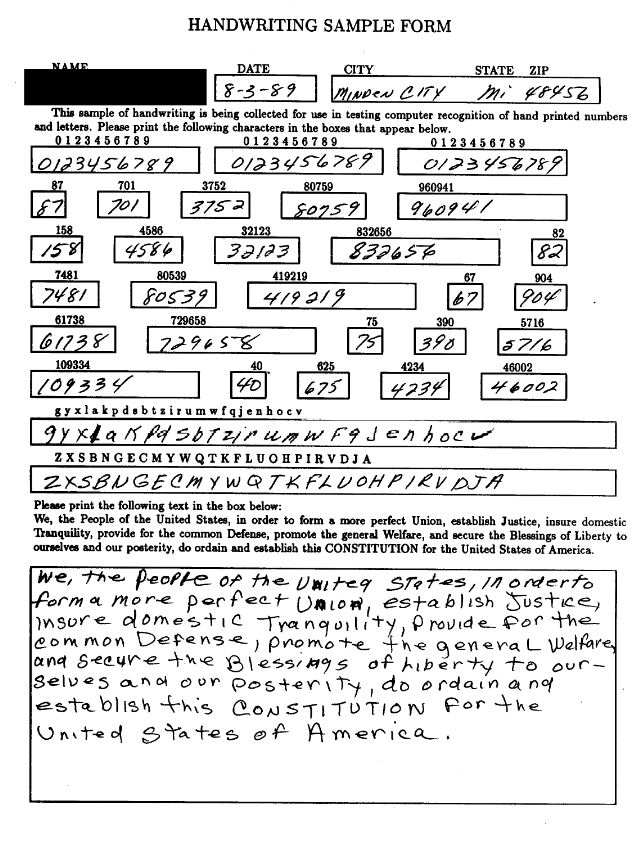
\includegraphics[width=0.6\linewidth]{images/sd19}
	\caption{NIST SD19 сангийн гар бичмэл тэмдэгтүүд цуглуулах зорилготойгоор бэлдсэн маягт. Гараар бөглөх 33 хэсгүүдтэй ба нэр, огноо оруулах нүднээс бусад хэсгүүд боловсруулагдана.}
	\label{fig:sd19}
\end{figure}

Цуглуусан өгөгдлөө by\_write, by\_field, by\_class, by\_merge хэмээх дөрвөн өөр төрлөөр ангилсан бөгөөд өгөгдлүүдээ хадгалахдаа дараах файлын төрлүүдээр хадгалсан. Үүнд:
\begin{itemize}
	\item .mis\footnote{Multiple Image Set} ялган авсан тэмдэгтийн зургуудыг хадгалах файлын төрөл
	\item .pct бүтэн хуудас маягтын зургийг хадгалах файлын төрөл
	\item .cls 62 ялгаатай төрлийн тэмдэгтүүдийн холбогдох зургийн мэдээллийг хамт хадгалж буй файлын төрөл
	\item .mit маяг бөглөсөн хүний мэдээллийг холбогдох тэмдэгтүүдийн мэдээлэлтэй хамт хадгалж буй файлын төрөл
\end{itemize}

Эхний хувилбараасаа хойш 2016 оны 9 сард санг хадгалах файлын төрлийг PNG форматтай болгон шинэчилж дахин шинэ хувилбар гаргажээ.

\subsection{MNIST \cite{mnist}}

Анх 1998 онд дээр дурдсан NIST -н Special Database 1 болон 3 дахь хувилбаруудын 0 -с 9 хүртэл 10 төрлийн тэмдэгтүүдтэйгээр танилцуулагдсан бөгөөд өнөөдрийг хуртэл оюун ухаан, хиймэл оюуны салбарт хамгийн түгээмэл ашиглагддаг сан яах аргагүй мөн билээ.

NIST анхлан SD-3 нь сургалтанд, NIST SD-1 нь тестэд зориулан зохион байгуулсан бөгөөд учир нь сургалтанд зориулсан өгөгдлүүд нь нөгөөхөөсөө хамаагүй цэвэрхэн, сайн боловсруулагдсан, амар танигдахаар байсан бол SD-1 нь ахлах сургуулийн сурагчдаар бөглүүлсэн маягтаас боловсруулагдсан байсан юм. Тийм ч учраас эдгээрх сангуудыг тэнцүү хуваан, дахин зохион байгуулж сургалтын 60000, тестийн 10000 зурагтай MNIST (Modified NIST) -г үүсгэсэн байна.\cite{mnist-paper}

\begin{figure}[H]
	\centering
	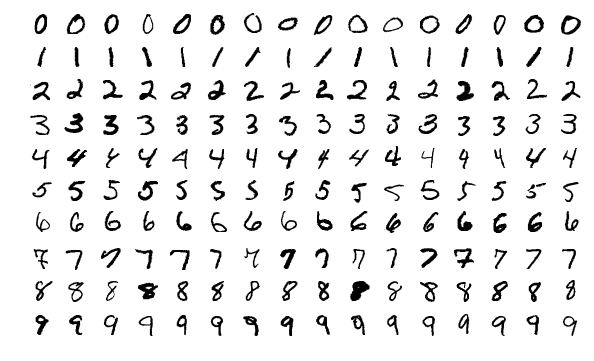
\includegraphics[width=0.9\linewidth]{images/mnist}
	\caption{MNIST сангийн жишээ тэмдэгтүүд \cite{mnist}}
	\label{fig:mnist-sample}
\end{figure}

NIST -н оролтын хоёртын зургуудыг эхлээд 20х20 хэмжээтэйгээр багасган боловсруулж үндсэн гурван хэлбэрээр туршсан. Эхнийх нь хэмжээг нь багасгасан зургуудынхаа төвийг олон, харьцааг алдагдуулахгүйгээр 28х28 дотор багтаасан. Хоёр дахь хувилбарт оролтын зургуудын налалтыг арилган тэгшлээд 20х20 хэмжээтэй болгон багасгаж deslanted буюу налууг арилгасан санд ашигласан. Харин сүүийн хэлбэр нь зургуудын хэмжээг нь 16х16 болгон багасгаж ашигласан.

Өнөөдөр MNIST сан нь дээрх төрлүүдийн хамгийн эхний хэлбэрээр вектор, олон хэмжээст матриц хадгалахад амар IDX гэх файлын төрөлтэйгөөр ашиглагдаж байгаа билээ.

\subsection{EMNIST \cite{emnist}}

Extended Modified NIST буюу EMNIST нь аль хэдийн MNIST санг ашиглаж байгаа алгоритм, системүүд ямар ч асуудалгүйгээр авч ашиглах боломжтой байх илүү өргөтгөсөн нээлттэй санг үүсгэх зорилготойгоор танилцуулагдсан юм.

Оролтын зургийг боловсруулах дараалал нь ерөнхийдөө MNIST\cite{mnist} -г үүсгэх зорилгоор NIST\cite{nist19} -н өгөгдлүүдийг хэрхэн боловсруулсан аргатай ойролцоо ч зургийг жижигрүүлэхэд ашигласан алгоритм, арга зэрэг нь өөр байгаа юм. Зурган дээр хувиргалт хийхдээ эхлээд зургийн урт, өргөнөөс хамгийн их хэмжээгээр хамгийн жижиг багтаасан тэгш өнцөгтийг тооцоолж хоосон үлдсэн хэсэгт дүүргэлт хийснээр урт, өргөнийг тэнцүүлэн дөрвөлжин зураг үүсгэсэн. Зургийн хэсгүүдийг захын ирмэгүүдэд наалдуулахгүйн тулд мөн 2 пикселийн хүрээг нэмжээ. Эндээс зургаа bi-cubic interpolation алгоритм ашиглан 28х28 хэмжээтэй болгон жижигрүүлсэн байна. Зураг \ref{fig:emnist-conversion}.

\begin{figure}[H]
	\centering
	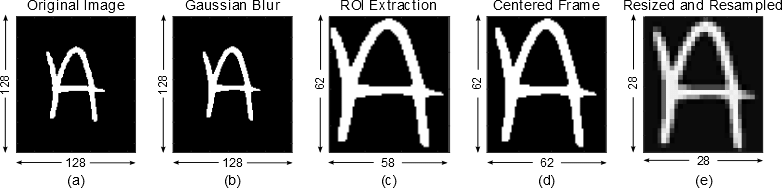
\includegraphics[width=1\linewidth]{images/emnist}
	\caption{EMNIST санг үүсгэхэд NIST сангийн зургуудыг боловсруулахад ашигласан хувиргалтын дараалал \cite{emnist}}
	\label{fig:emnist-conversion}
\end{figure}

Машин сургалтанд зориулагдсан сангууд сургалтын болон тестийн гэх хоёр хэсэгт хуваагддаг бөгөөд EMNIST -н хувьд NIST -н өгөгдлийг боловсруулахдаа MNIST -н баримталсан аргыг буюу Census Bureau -н ажилчид, ахлах сургуулийн сурагчдаас цуглуулсан тэмдэгтүүдийг сургалт болон тестийн өгөгдөлдөө тэнцүү хуваан, тестийн өгөгдөл үүсгэхдээ тэдгээрээс санамсаргүй аргаар сонгон авч үүсгэжээ.

\subsection{IAM \cite{iam-database}}

Англи хэл дээрх хамгийн түгээмэл ашиглагддаг сангуудын нэг нь IAM\footnote{Institut für Informatik und angewandte Mathematik ( = Компьютерийн ухаан, хэрэглээний математикийн тэнхим), Берны их сургууль, Берн, Щвейцарь} сан бөгөөд дээр дурдсан сангуудаас ялгаатай нь үндсэн өгөгдөл нь дан гараар бичигдсэн бүтэн өгүүлбэрээс цуглуулагдсан буюу LOB corpus \cite{lob-corpus}\footnote{Lancaster-Oslo болон Bergen сургуулиудын хамтран боловсруулсан сан \url{http://korpus.uib.no/icame/manuals/LOB/INDEX.HTM}} дээр суурилж энэхүү сан боловсруулагдсан. LOB corpus -н анхны хувилбар 1970 онд танилцуулагдсан бөгөөд 400 гаруй хүний 1066 гараар бөглөгдсөн маягтаас авсан 10841 ялгаатай үгсийг агуулдаг.

\section{Судалгаанаас хийсэн дүгнэлт}

Өнөөдөр машин сургалт, гар бичмэл танилтын судалгаануудад хамгийн нийтлэг ашиглагддаг англи хэлний дөрвөн сангуудад судлагаа хийж үзээд дараах дүгнэлтүүдийг гаргалаа. Үүнд:

\begin{itemize}
	\item Сан нь хэрхэн зохион байгуулагдсан, өгөгдлүүд ямар форматтайгаар хадгалагдсан, авч ашиглах, хувиргах боломжууд нь энэ чиглэлээр судалгаа хийж буй хүмүүсийн дунд тархах, түгээмэл ашиглагдахтай шууд холбоотой. Иймээс санг авч ашиглах, өгөгдлүүдийг хувиргахад амар байх
	\item MNIST болон EMNIST нь энэ чиглэлийн сургалт, судалгаа, шинэ төслүүдэд хамгийн түгээмэл ашиглагдаж буй сан мөн бөгөөд үүнтэй холбоотойгоор эдгээр сангуудыг ашигладаг олон систем, програм хангамжууд байгаа учир өөрийн үүсгэж буй сангаа эдгээр сангуудтай нийцтэй ажиллах боломжтой байдлаар зохиомжлох\label{criteria:mnist-compatible}
	\item Өөрийн сангаас хүмүүст авч ашиглахад амар байлгах үүднээс мөн боломжит дэд сангууд (subset) нэмэлтээр үүсгэх
	\item Сангийн сургалтын болон тестийн өгөгдлүүдийг хэрхэн ялгаж, зохион байгуулах нь чухал бөгөөд гаргацтай зургууд, танихад хэцүү зургуудыг аль аль талд тэнцүү байдлаар хуваан зохион байгуулах
\end{itemize}
